\section{Foundations}
\label{sec:Foundations}

\NOTE{\emph{Length:} 2 p., \emph{Responsible:} Tony}
\NOTE{Based on BX 2017 paper, Section~3.1. Should include the taxonomy of Figure~3.}

\subsection{Input and Output Data}

\definition[Model]~\\
$A$, $A'$, $B$, $B'$

\definition[Delta]~\\
$\delta: A \rightarrow A'$

\definition[Operational Delta]~\\
$(\delta): A \stackrel{@}{\rightarrow} A'$

\definition[Edit]~\\
$@: M \rightarrow \Delta$\\
$@: A \longmapsto (\delta): A \stackrel{@}{\rightarrow} A'$

\definition[Structural Delta]~\\
$\langle\delta\rangle: A \Rightarrow A'$

\definition[Model Space]~\\
$\mathcal{M}_S = (\Delta_S, M_S), \mathcal{M}_T = (\Delta_T, M_T)$

\definition[Corr]~\\
$\sigma : A \leftrightarrow$ B

\definition[Triple Space]~\\
$(\mathcal{M}_S, \mathcal{M}_T, C \subseteq R)$


\subsection{Basic Operations}

\begin{figure}[tb!]
	\centering
	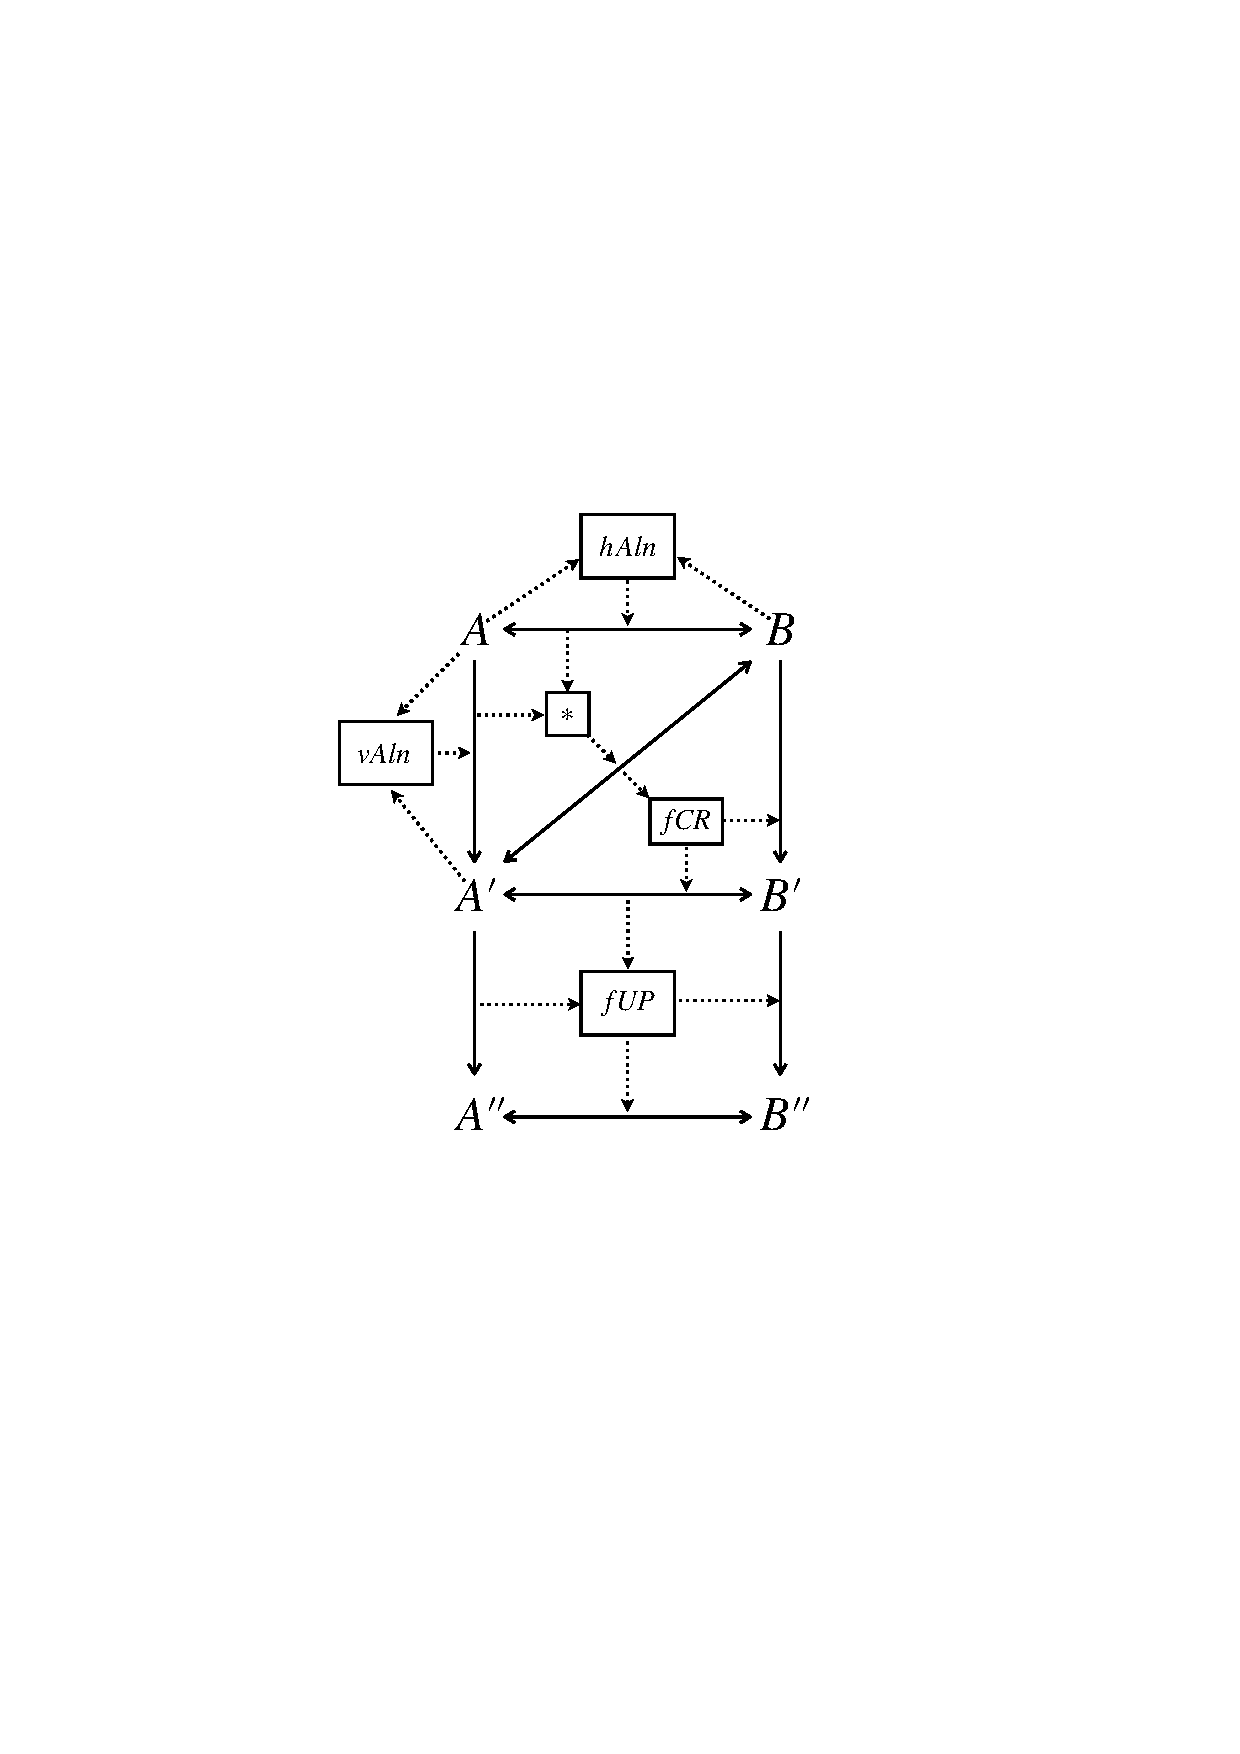
\includegraphics[width=0.55\columnwidth]{diagrams/BasicOperationsOverview}
	\caption{Overview of basic operations}
	\label{fig:basicOperationsOverview}
\end{figure}

\subsection{BX Tool Architectures}

\begin{figure}[tb!]
	\centering
	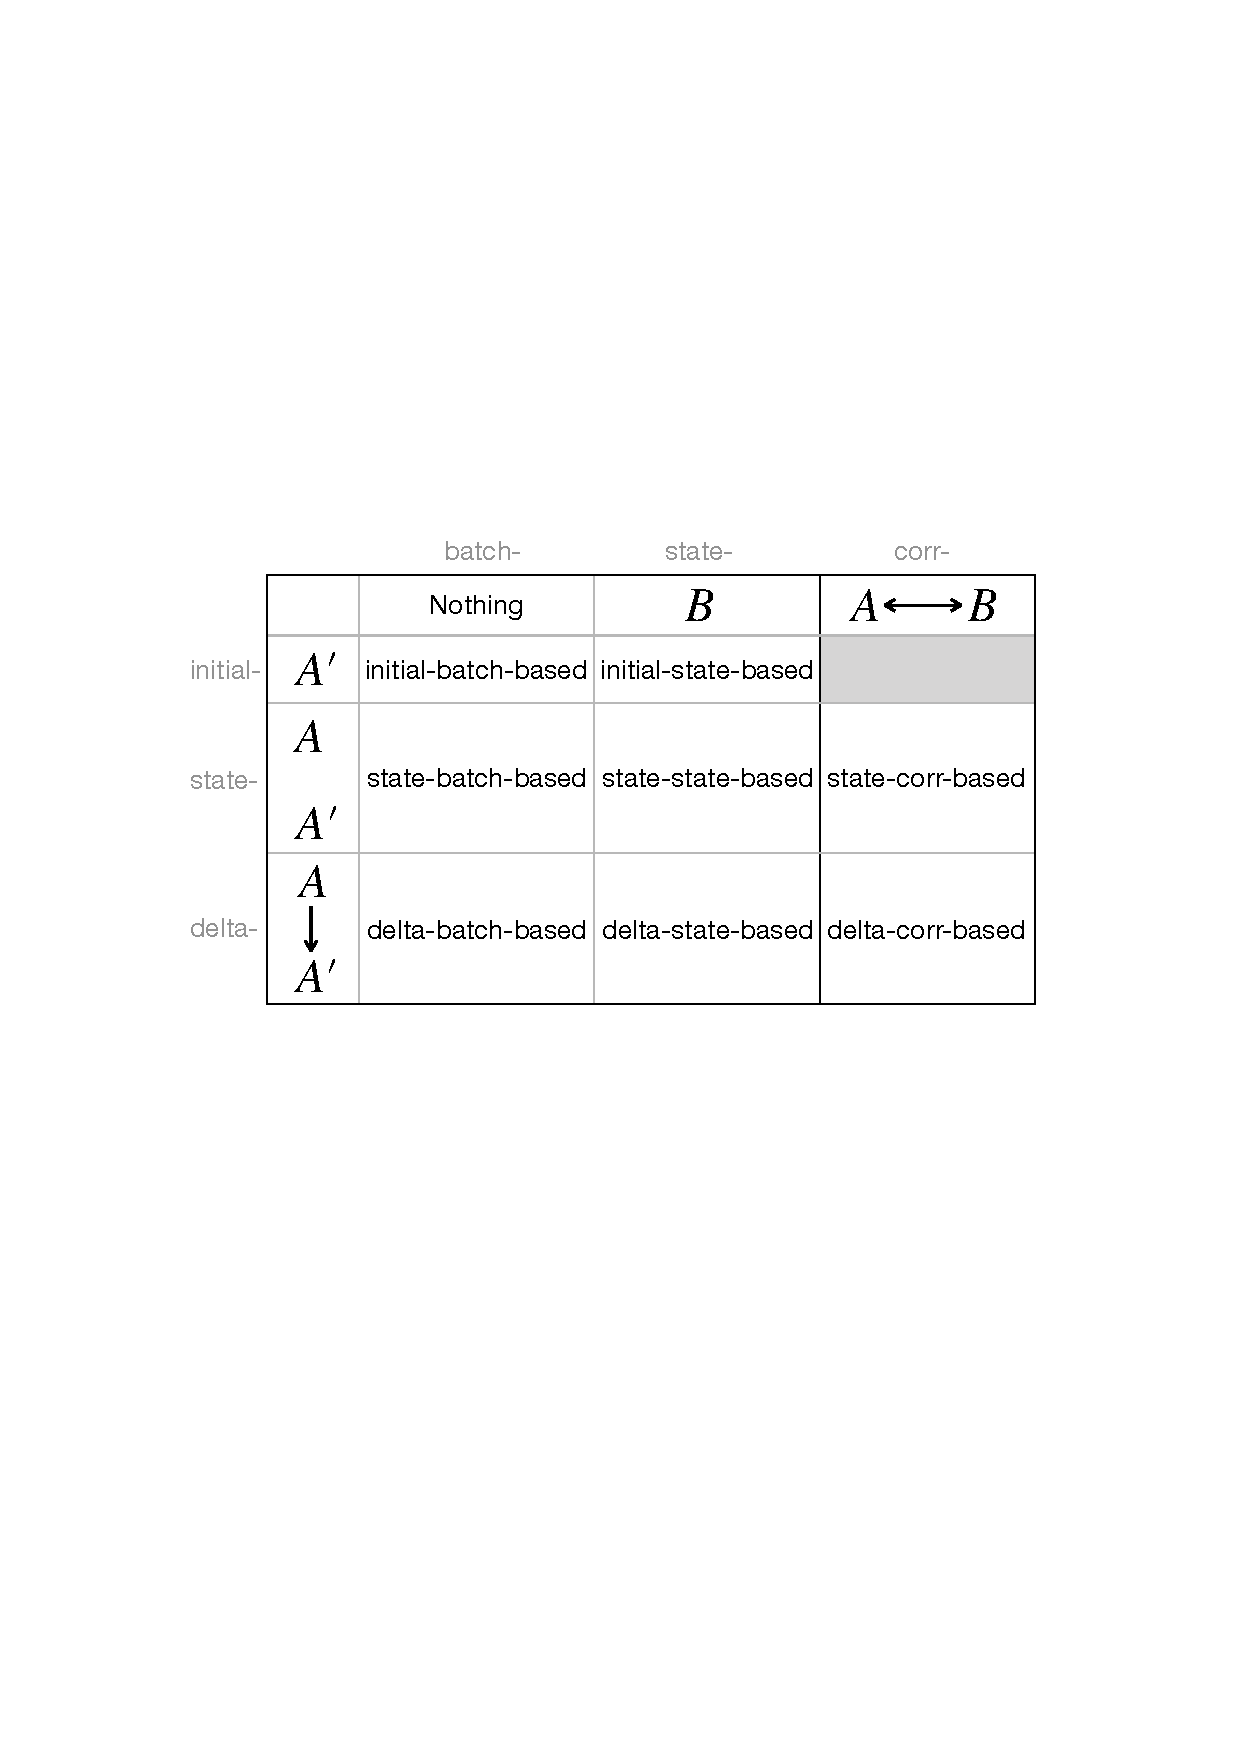
\includegraphics[width=0.9\columnwidth]{diagrams/ArchitectureLandscape}
	\caption{Overview of bx tool architectures}
	\label{fig:architectureLandscape}
\end{figure}

\begin{figure}[tb!]
	\centering
	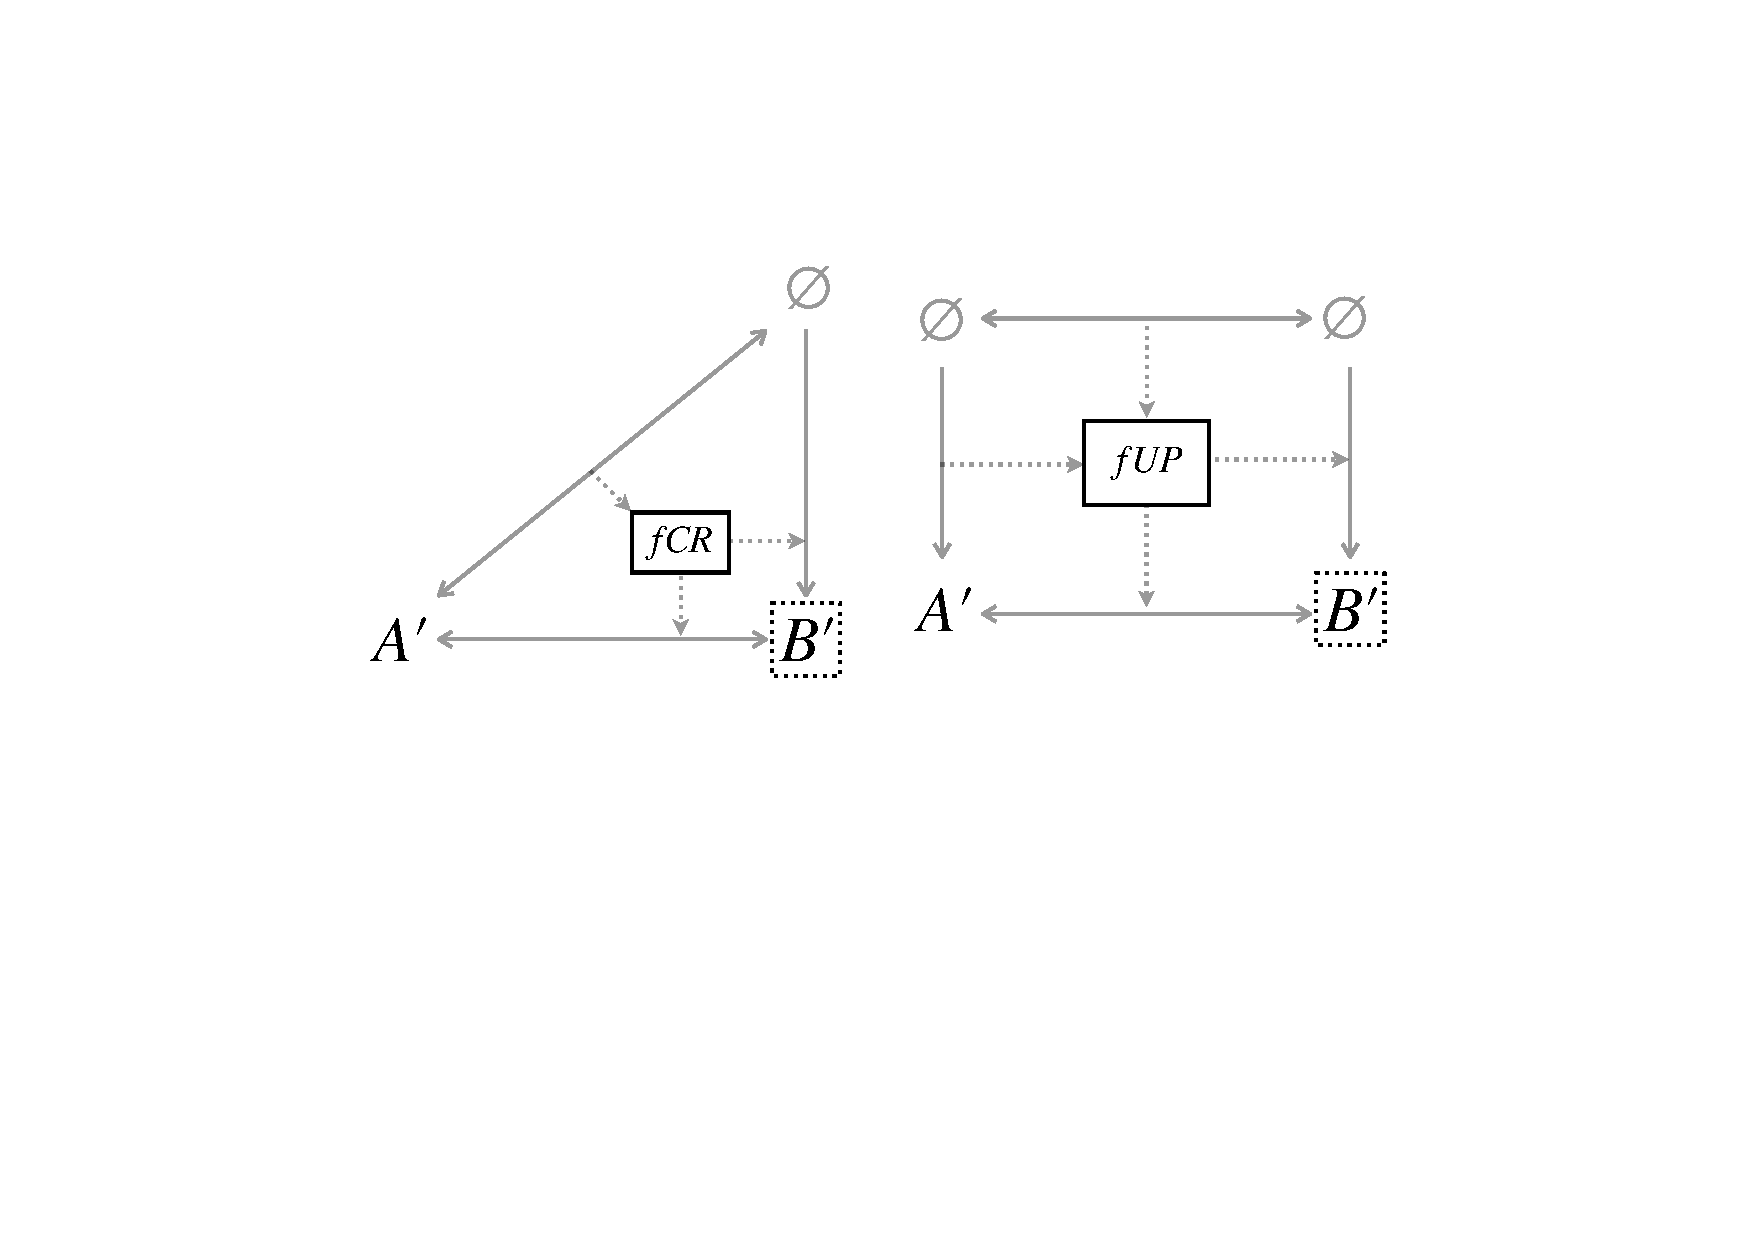
\includegraphics[width=0.8\columnwidth]{diagrams/initial-batch-based}
	\caption{Initial-batch-based Architecture}
	\label{fig:initialBatchBased}
\end{figure}

\begin{figure}[tb!]
	\centering
	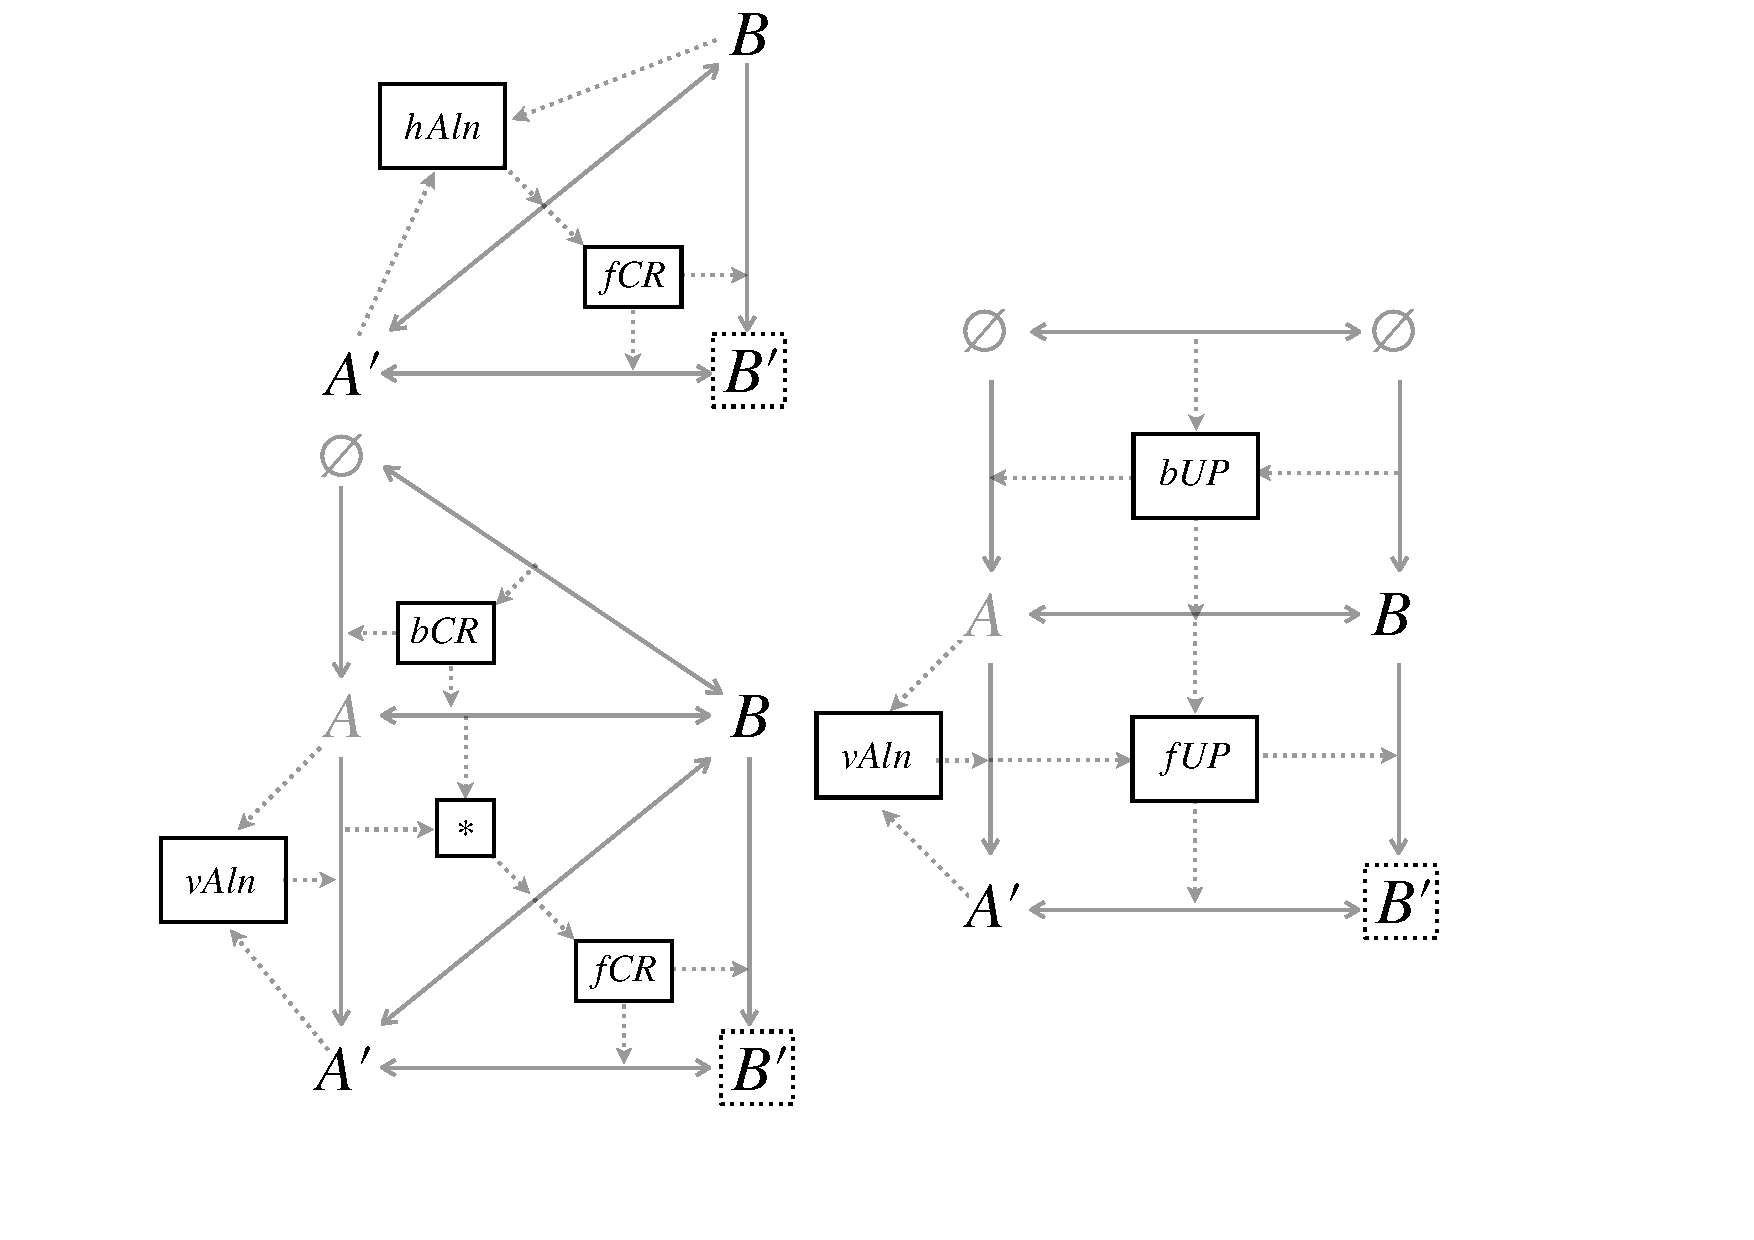
\includegraphics[width=\columnwidth]{diagrams/initial-state-based}
	\caption{Initial-state-based Architecture}
	\label{fig:initialStateBased}
\end{figure}

\begin{figure}[tb!]
	\centering
	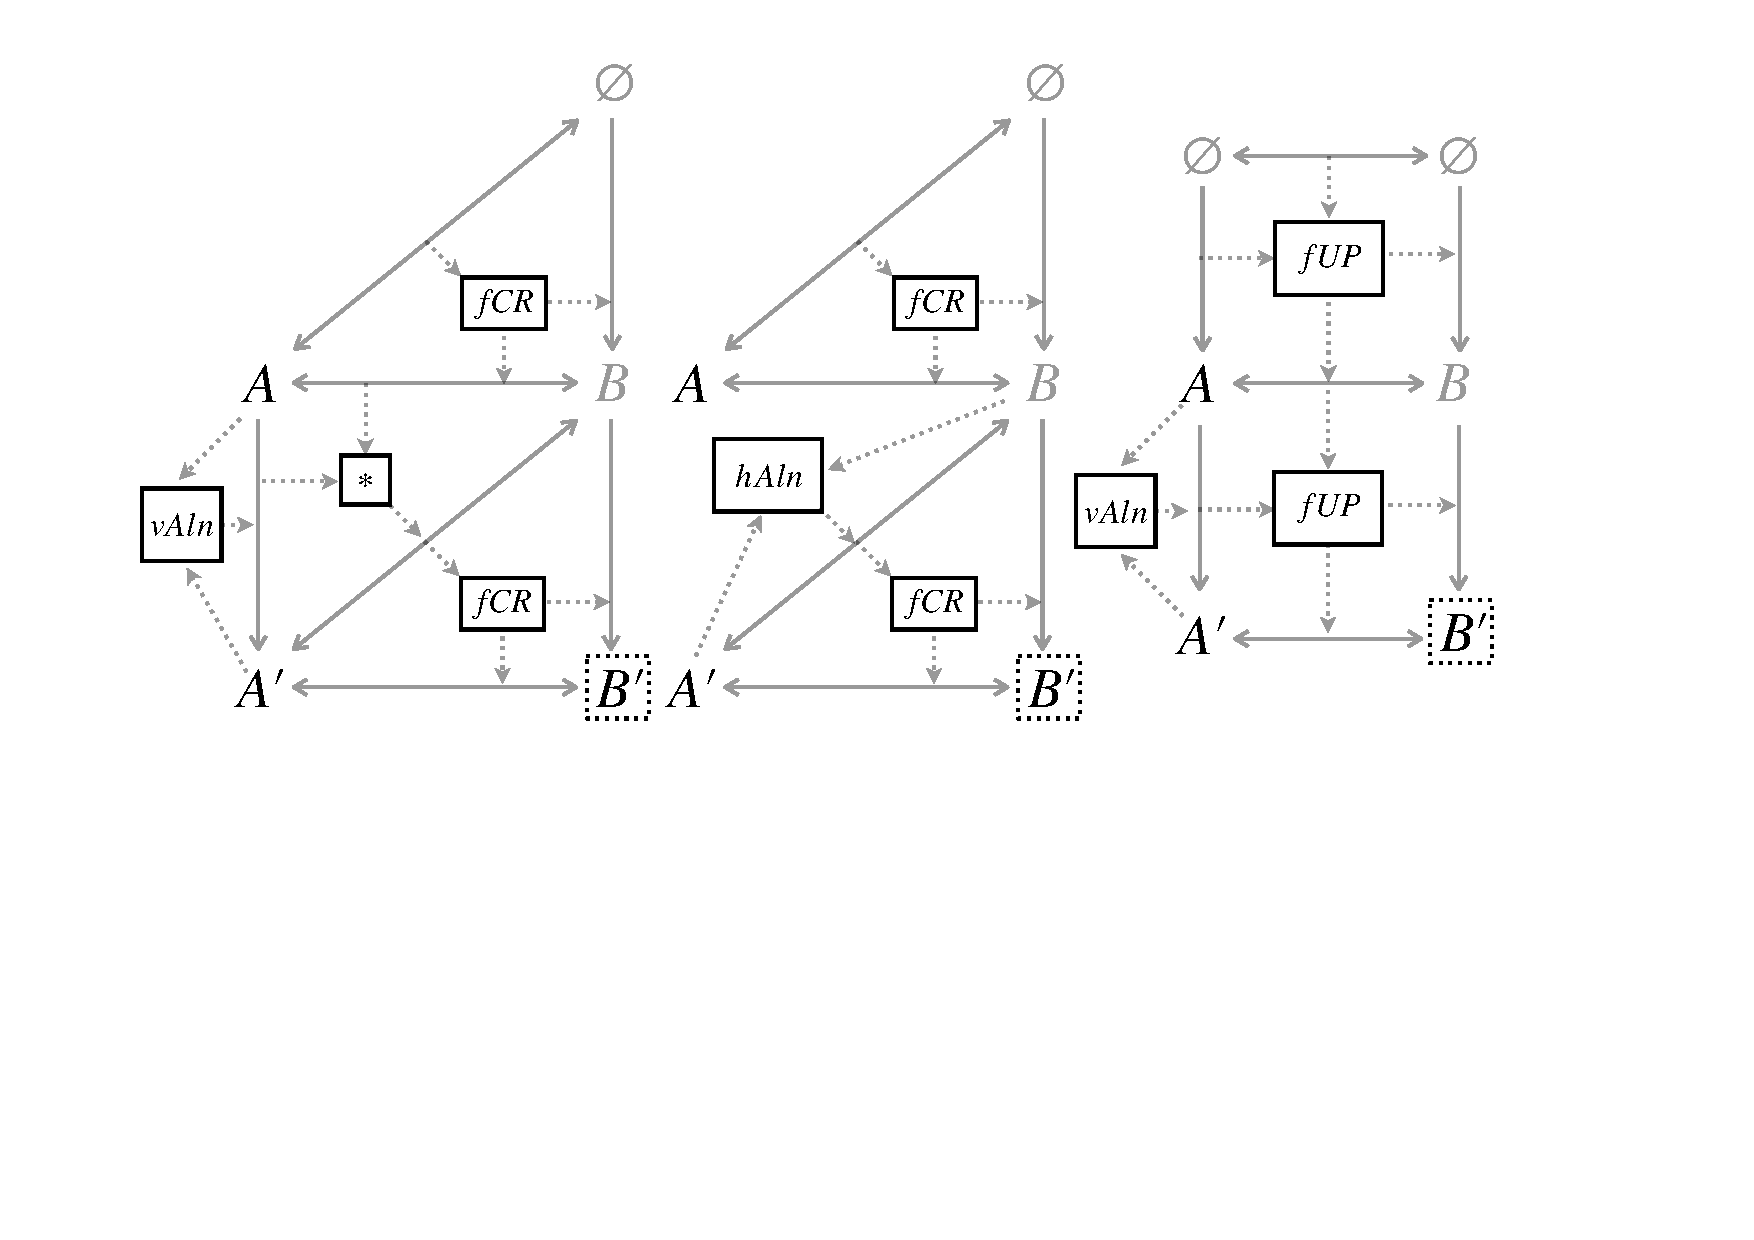
\includegraphics[width=\columnwidth]{diagrams/state-batch-based}
	\caption{State-batch-based Architecture}
	\label{fig:stateBatchBased}
\end{figure}

\begin{figure}[tb!]
	\centering
	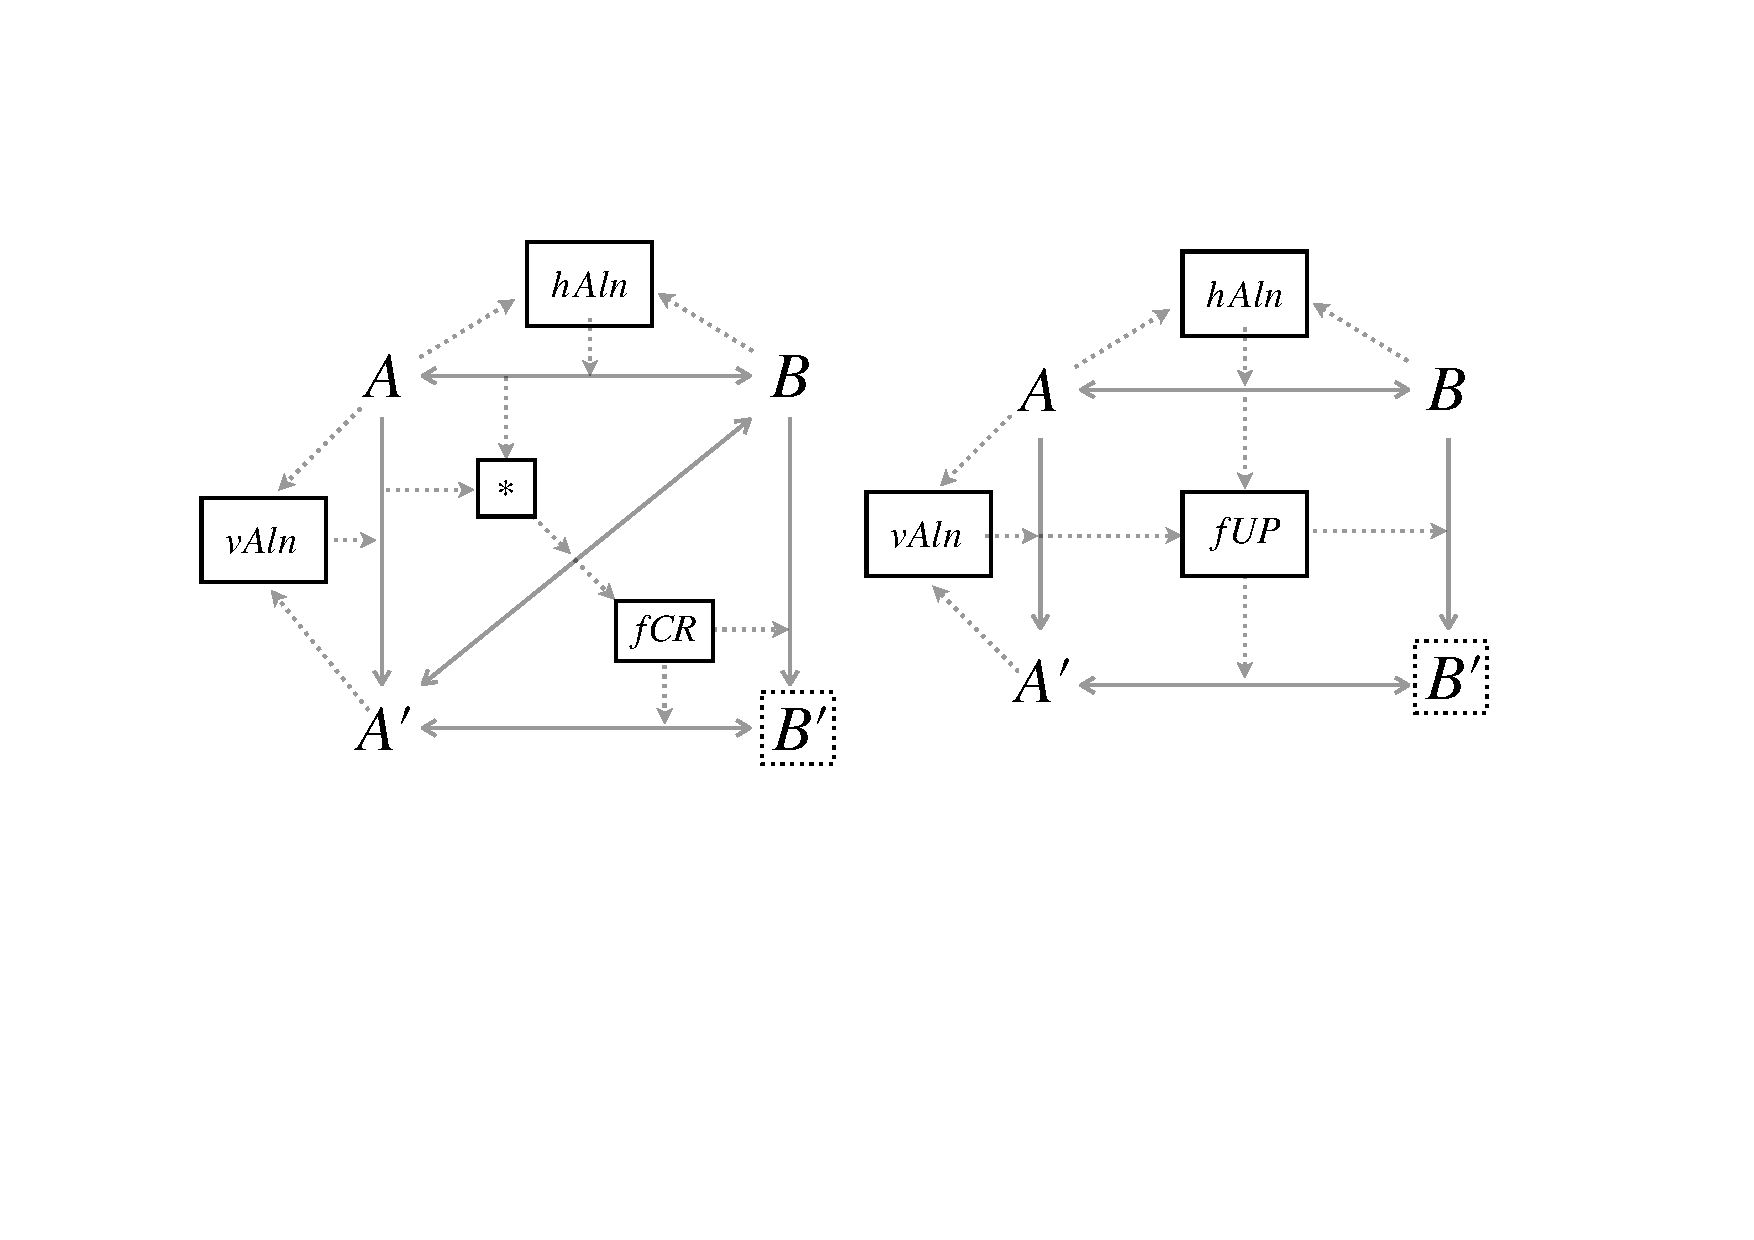
\includegraphics[width=\columnwidth]{diagrams/state-state-based}
	\caption{State-state-based Architecture}
	\label{fig:stateStateBased}
\end{figure}

\begin{figure}[tb!]
	\centering
	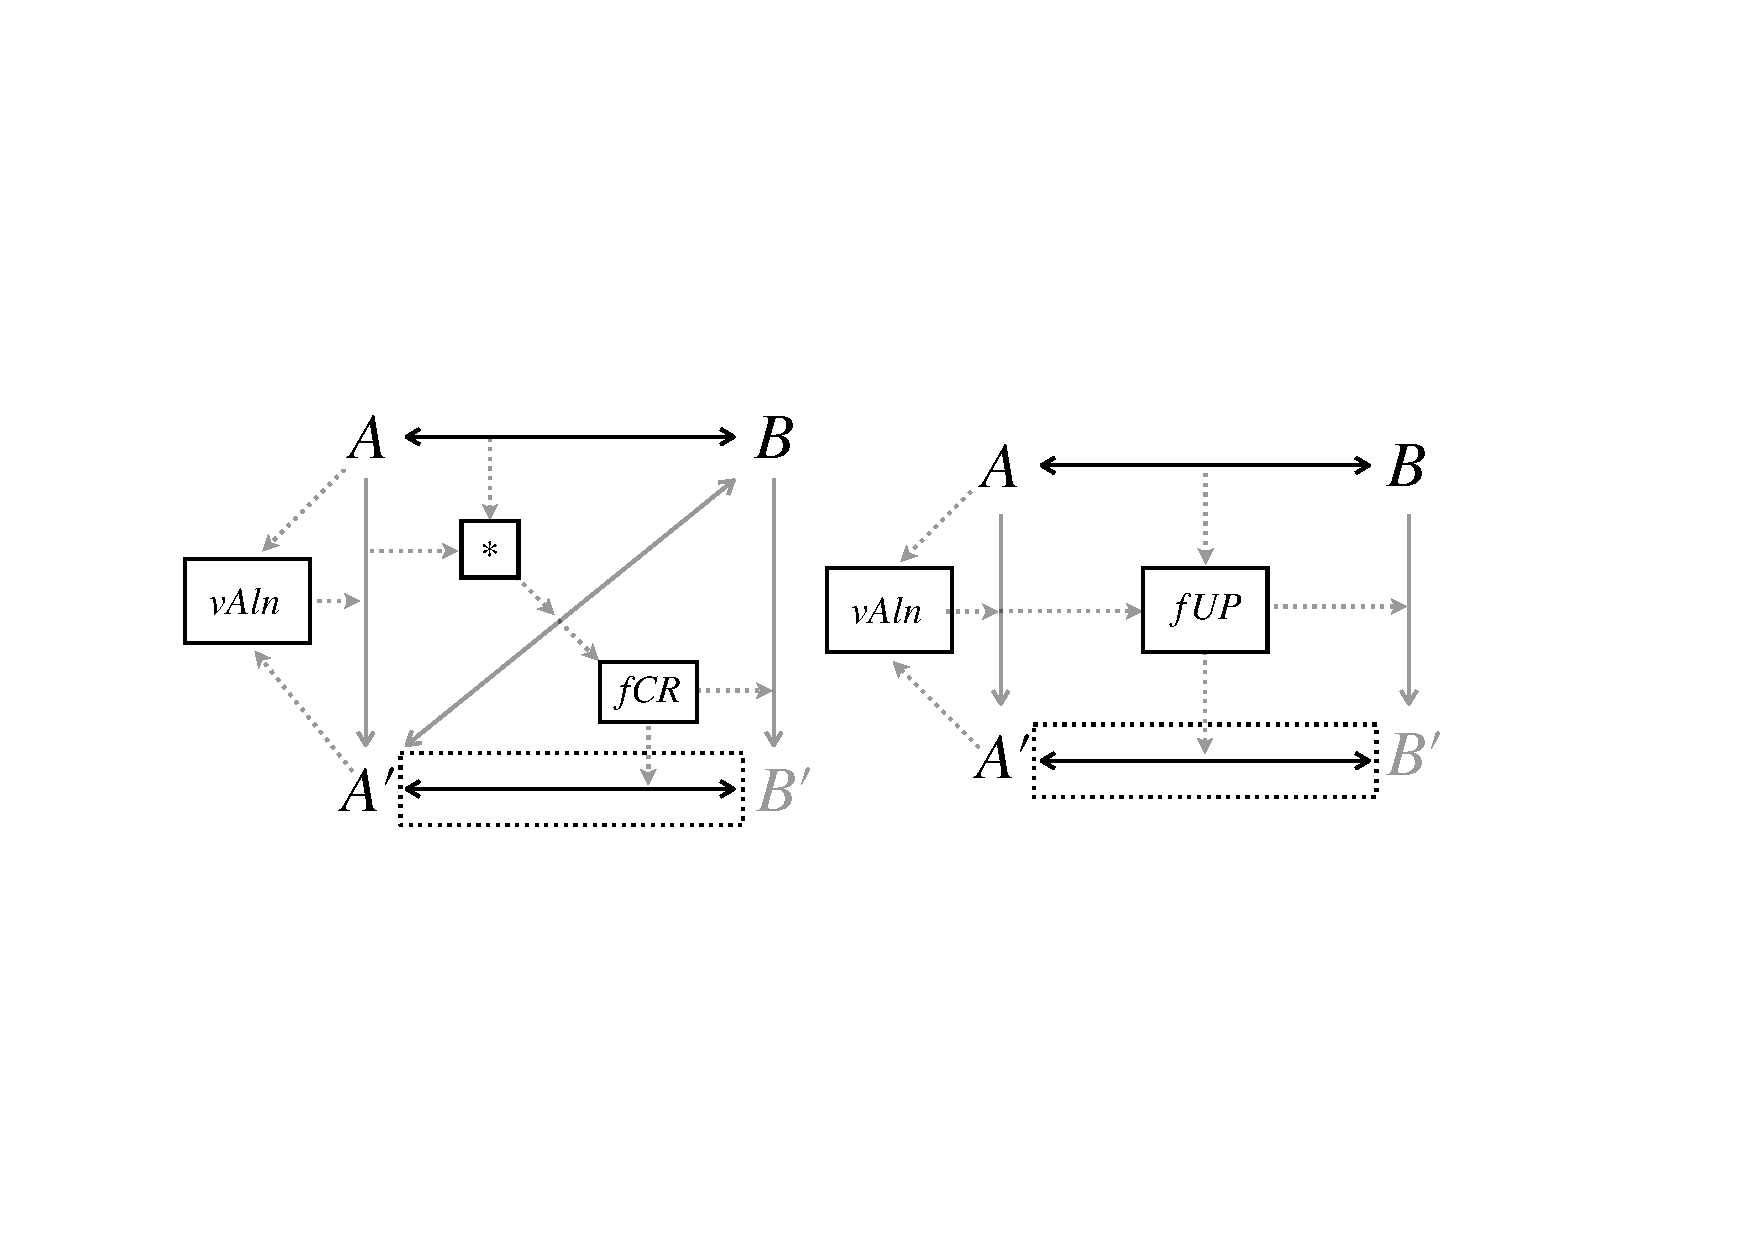
\includegraphics[width=\columnwidth]{diagrams/state-corr-based}
	\caption{State-corr-based Architecture}
	\label{fig:stateCorrBased}
\end{figure}

\begin{figure}[tb!]
	\centering
	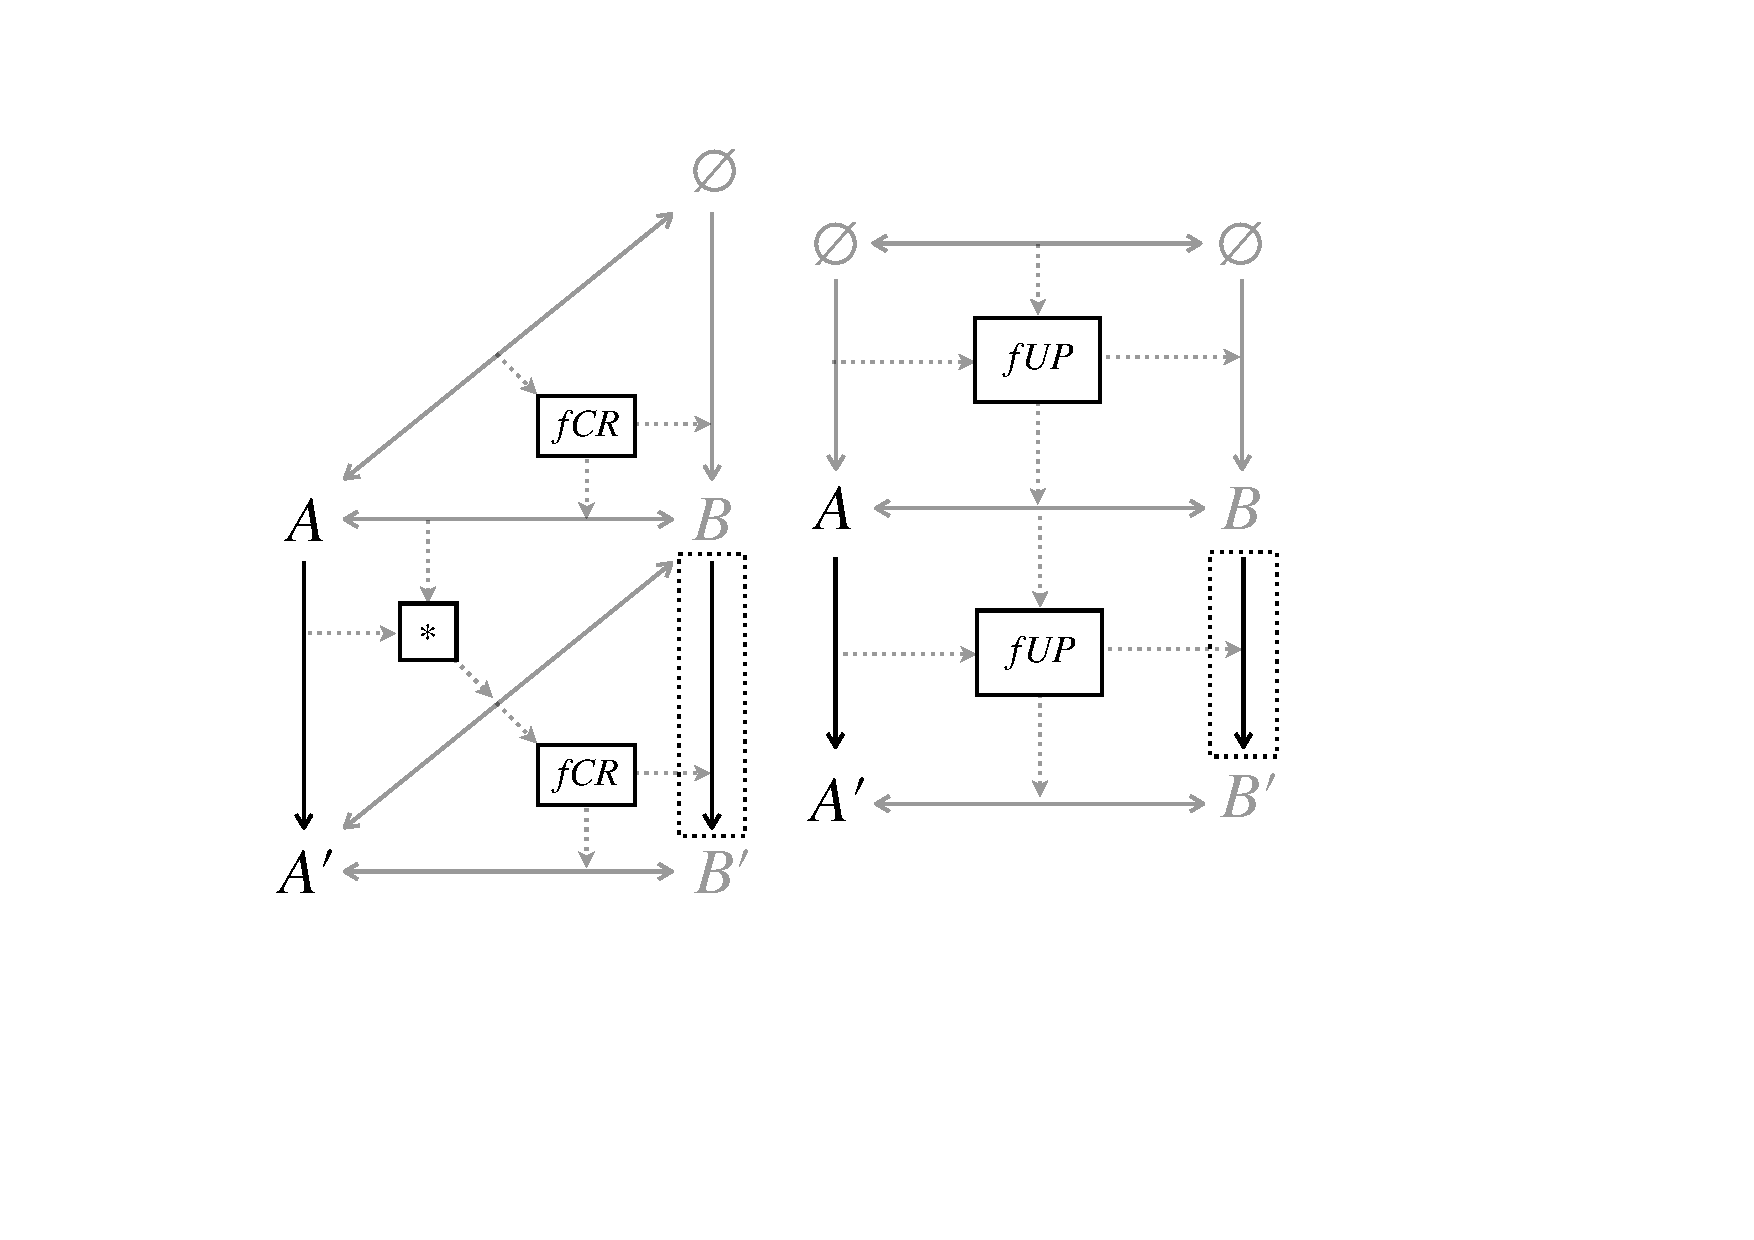
\includegraphics[width=0.73\columnwidth]{diagrams/delta-batch-based}
	\caption{Delta-batch-based Architecture}
	\label{fig:deltaBatchBased}
\end{figure}

\begin{figure}[tb!]
	\centering
	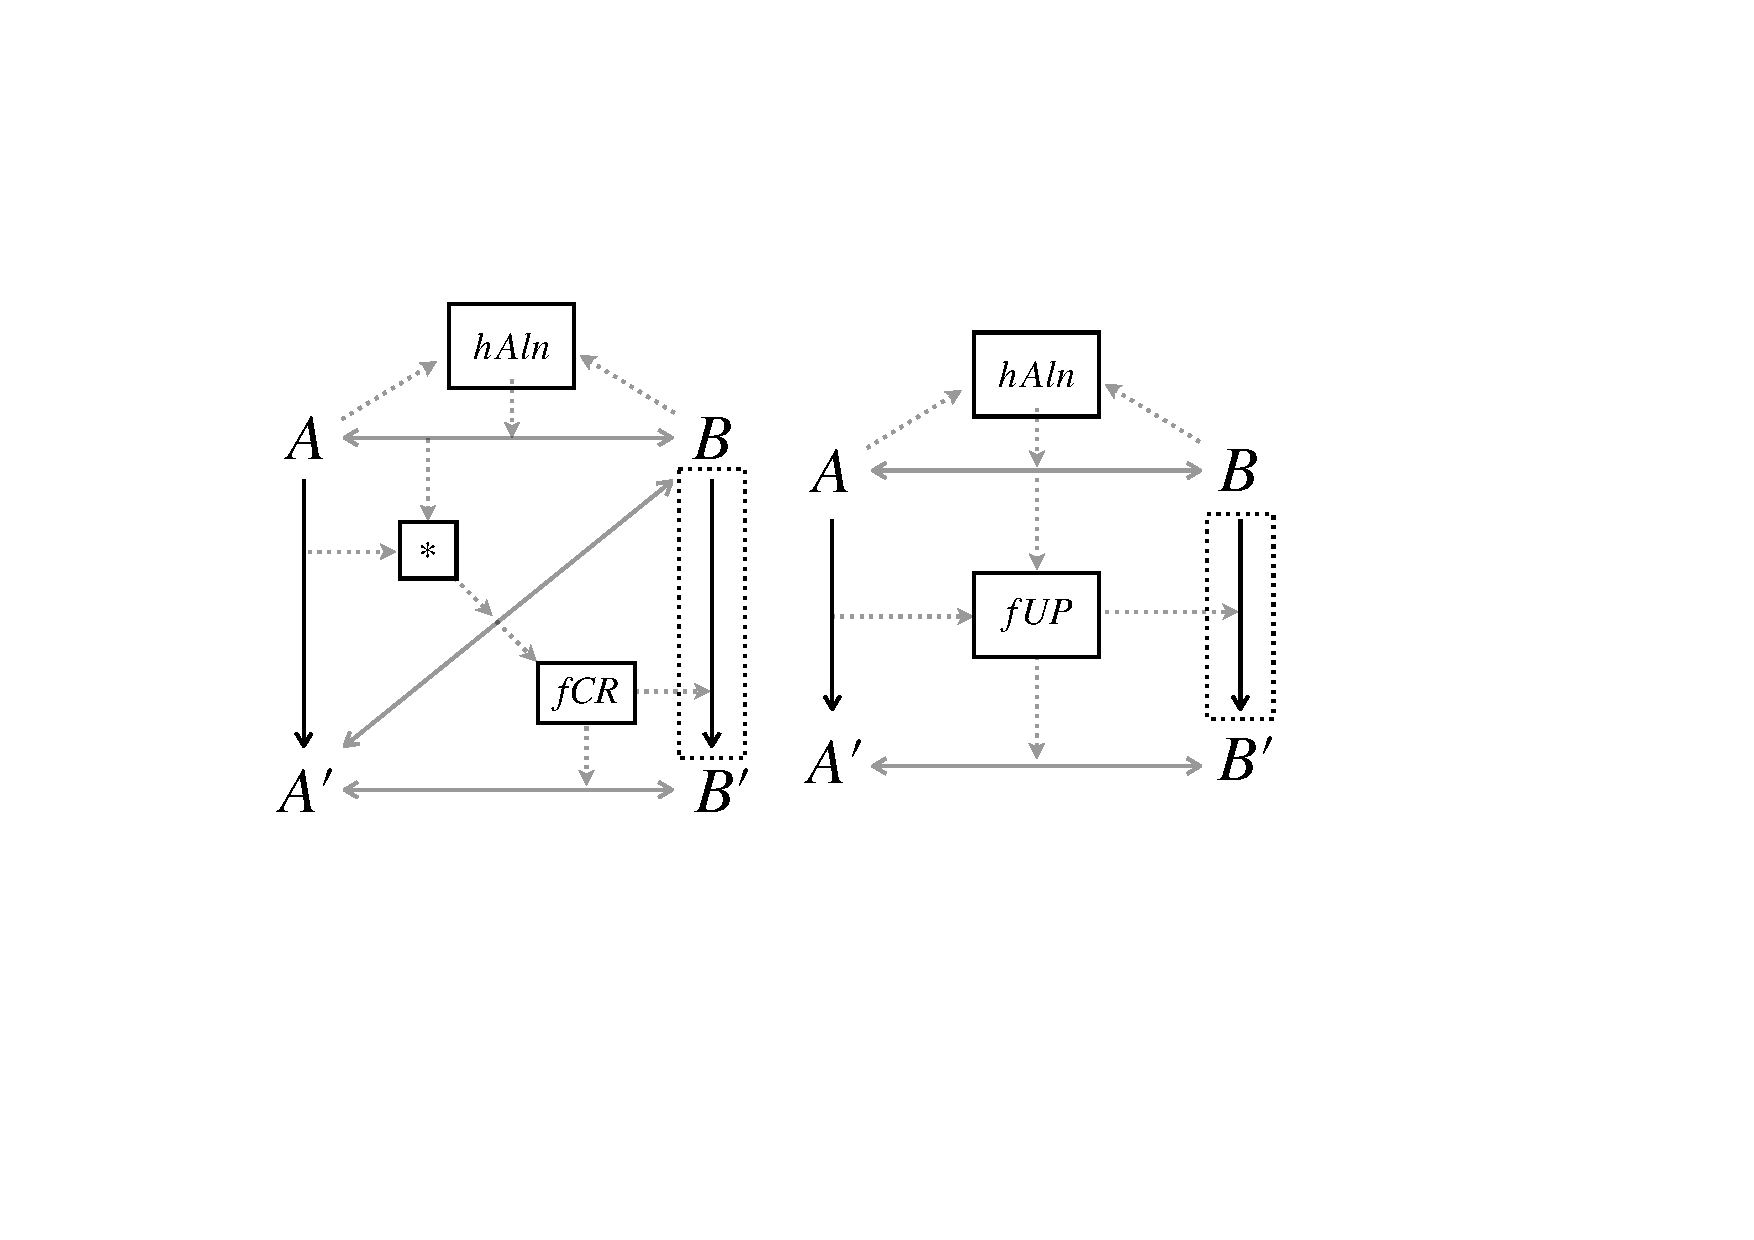
\includegraphics[width=0.75\columnwidth]{diagrams/delta-state-based}
	\caption{Delta-state-based Architecture}
	\label{fig:stateBatchBased}
\end{figure}

\begin{figure}[tb!]
	\centering
	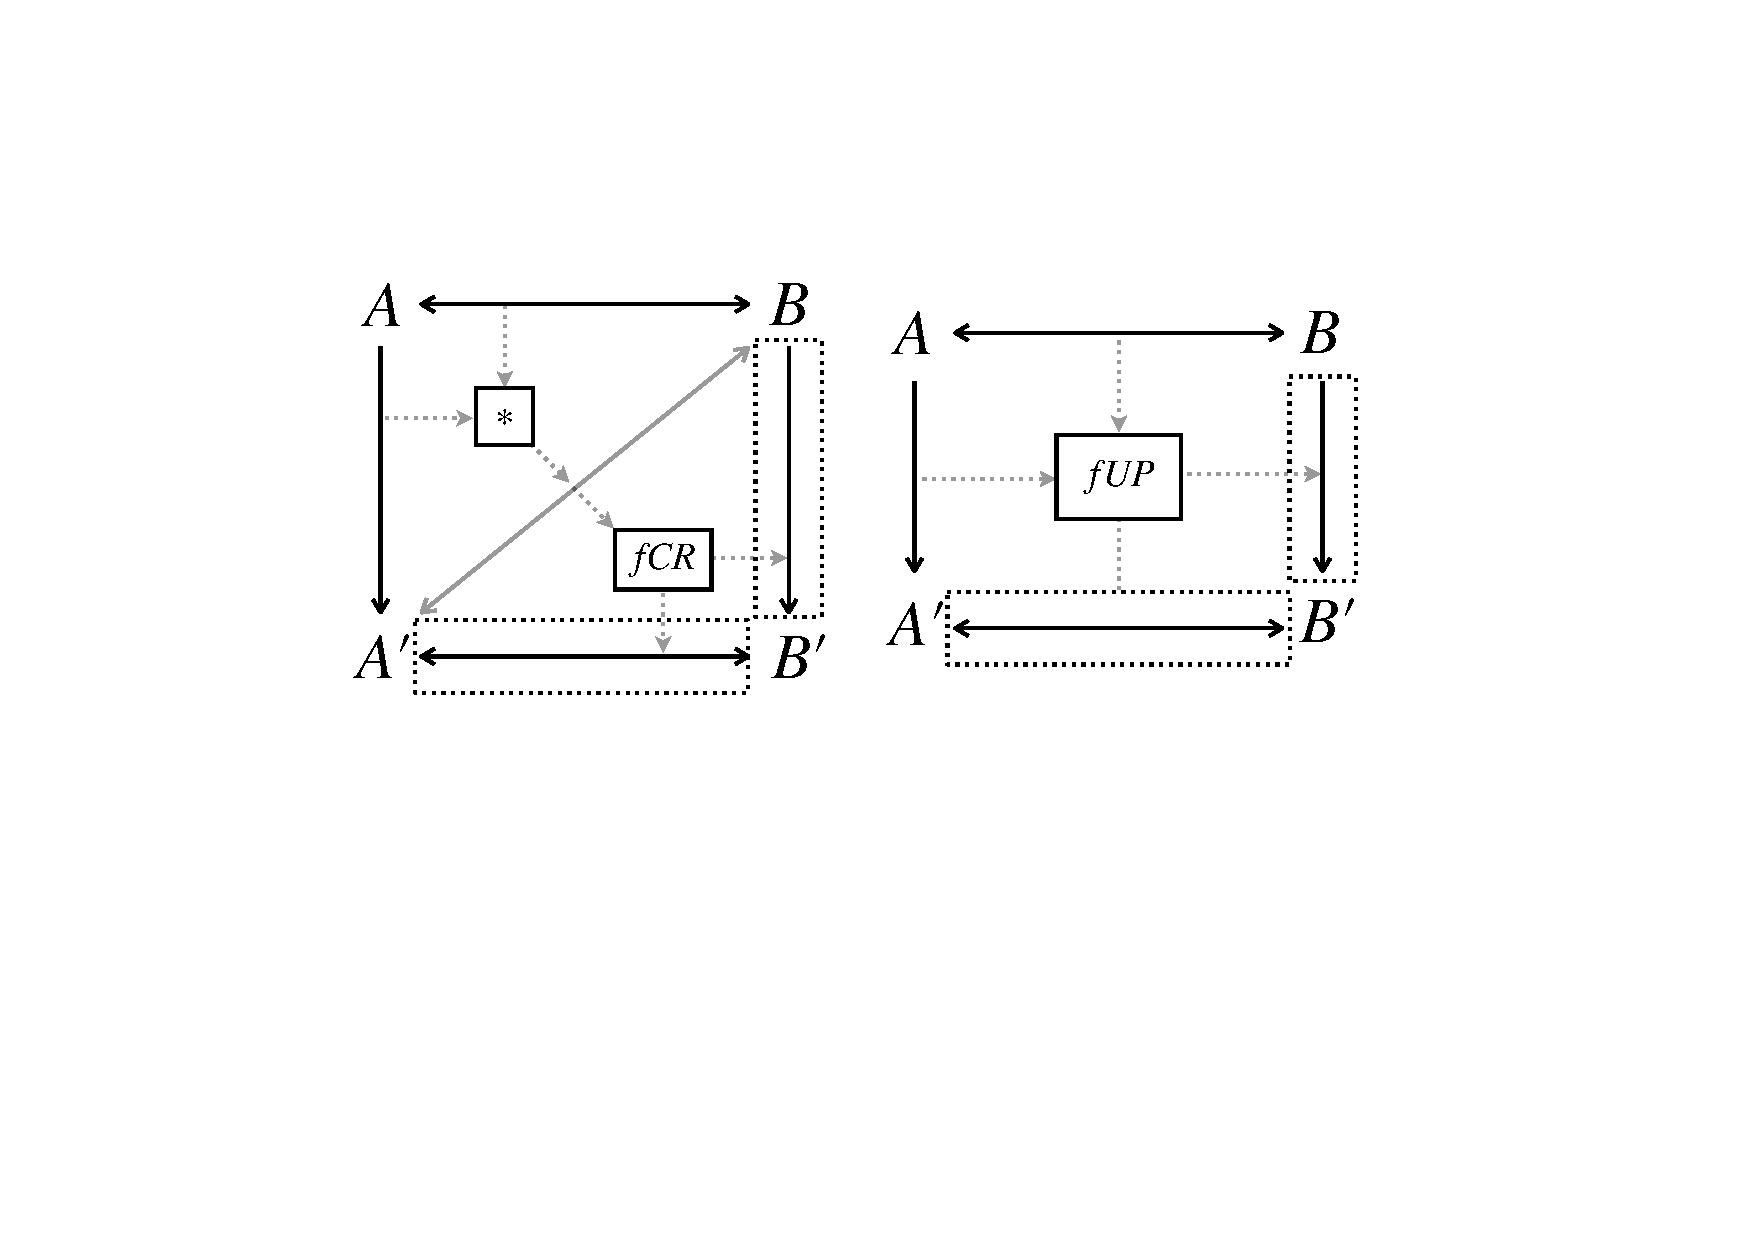
\includegraphics[width=0.75\columnwidth]{diagrams/delta-corr-based}
	\caption{Delta-corr-based Architecture}
	\label{fig:deltaCorrBased}
\end{figure}

\clearpage